In this section we study the performance of Capsule. Using simulated data, we compare Capsule to deterministic methods of event detection and show that Capsule outperforms them at identifying when events occur.  
%We also examine how sensitive Capsule is to the attributes of a dataset and model parameters.
We conclude by exploring three real-worlds datasets with Capsule.

\subsection{Performance}

We generated ten simulated datasets using our generative process.  Each dataset spans 100 days and contains content associated with ten entities.  Approximately ten events also exist in each dataset, randomly distributed in time and with a three day decay of relevancy.

To evaluate performance, we rank each day by its probability of having an event occur, and plot the number of true events discovered against the number of false positive events, as shown in Figure~\ref{fig:sim_auc}; the area under the curve (AUC) can be computed for a single evaluation metric.  Note that this approach is only valid when true events are known, and thus we only apply it to simulated data.

We compare Capsule to two baseline approaches: one considers the greatest document outlier on a given day--days with the furthest outliers are the most likely to have events.  The other approach is similar: days are represented by an average of all documents associated with that day, and one considers how these averages deviate from the global average--the further away, the more likely an event.

Figure~\ref{fig:sim_auc} shows that Capsule outperforms both of these approaches.  It should be noted that inference on Capsule will produce different results, depending on the random seed; the results shown are the best of three random seeds.

\begin{figure}[ht]
\centering
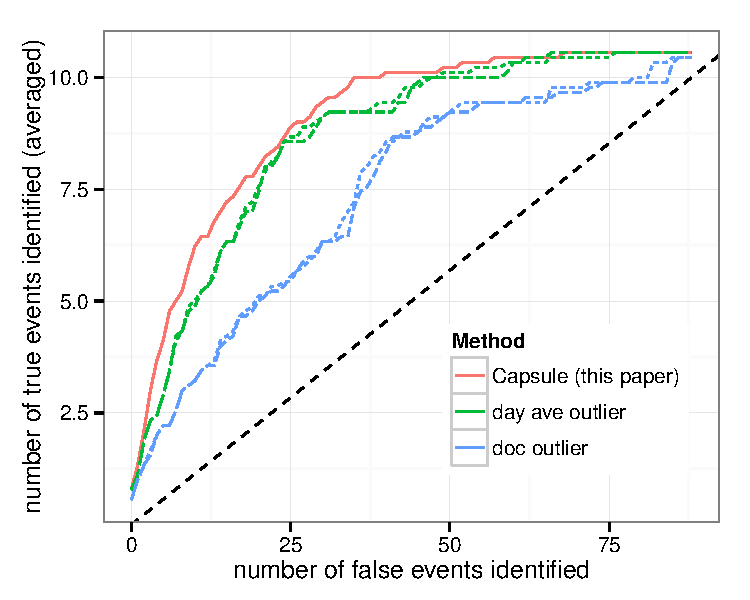
\includegraphics[width=\linewidth]{fig/sim_auc.pdf}
\caption{Average performance on ten simulated datasets; lines closer to the upper-left are better.  Baselines consider outliers based on full corpus averages (dashed) and averages of all entity documents (dotted).  Capsule performance is best of three random seeds.}
\label{fig:sim_auc}
\end{figure}


%\PP fig / discussion of varrying entity dists in simualted data

%\PP performance vs parameters (event occurrence hyperparameter (which impacts initialization), event duration)

\subsection{Exploration}

\parhead{Cables}
\PP where did we get it / size / preprocessing

\PP plot of events timeline with select real-world match evetns pointed out (verified by history lab)

\PP example interesting entities + figure

\PP explore pairwise entities? (quick with and single figure shared with enron); compare sender vs reiever for same pair  (or does direction matter?? tyr both ways) look at sender in norma model vs sender in a few pairs under this construction 

\parhead{arXiv}
\PP where did we get it / size / preprocessing

\PP plot of events timeline with select real-world match evetns pointed out (verified by history lab)

\PP example interesting entities + figure

\parhead{enron}
\PP where did we get it / size / preprocessing

\PP plot of events timeline with select real-world match evetns pointed out (verified by history lab)

\PP example interesting entities + figure

\PP explore pairwise entities?



% \parhead{Cables}
% We obtained around two million of these cables sent between 1973 and 1977 via the History Lab at Columbia,\footnote{http://history-lab.org} which received them from the Central Foreign Policy Files at the National Archives.  In addition to the text of the cables themselves, each document is supplemented with information about who sent the cable (e.g., the State Department, the U.S. Embassy in Saigon, or an individual by name), who received the cable (often multiple entities), and the date the cable was sent.
% Excerpts from three example cables are shown in Figure~\ref{fig:cables_example}.

% % \begin{figure}[ht]
% % \centering
% % 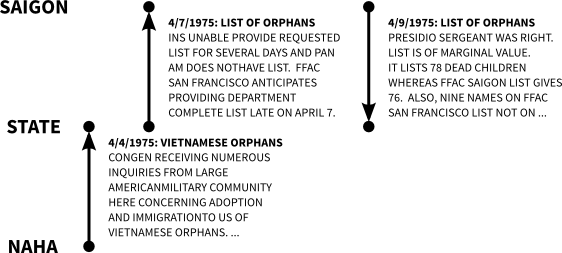
\includegraphics[width=\textwidth]{../fig/cables_orphan_example.png}
% % \caption{Example excerpts of cables sent in April 1975 concerning orphans from the Vietnam War.}
% % \label{fig:cables_example}
% % \end{figure}

% \parhead{arXiv}

% \parhead{Enron}


% \PP insert table and refetence for both (number of days, entities, total messages, or something); maybe a plot showing attributes of the data...somehow inform them that the state department is a bias for the cables data

% \PP footnote on handling multiple recipients of message...

% \subsection{Metrics and competing methods}

% \PP how we evaluate based on real events

% \PP how we evaluate based on perplexity (prediction of words)

% \PP competing methods for perplexity: LDA, average user words?, dynamic topic model, network topic models

% \subsection{Performance and exploration}

% \PP sumry of comparison to gold-standard events for cables

% \PP table of predictive likelihood results and summary pgh; and/or cite tea leaves paper

% \parhead{Exploration}

% \PP charachetrize events manually (based on cables) vs event detection characterization

% \PP show descriptions for cables entities and select events; same for arxiv/enron

% \PP any other exploration you can think of!


% Results: ROC curve (x=false postive rate, y=true postive rate)